\chapter{Rhythm and meter}
\label{sec:rhythm-and-meter}

\subsection*{What you can do after this chapter}
\begin{itemize}
  \item Count the pulse in a piece of music and say whether it is 4/4, 3/4, or 6/8.
  \item Read note values, dots, ties, and rests, and convert ``how long'' into beats and seconds.
  \item Hear and write basic syncopation and backbeat instead of placing every note on the downbeat.
  \item In Yeban, set tempo, time signature, ruler, quantization, and metronome to one consistent grid before writing rhythm.
\end{itemize}

\subsection{Pulse, beat, and tempo}

Music first has a pulse; organizing that pulse into equal intervals gives beats. Grouping beats gives bars. The time signature tells you how many beats per bar; tempo tells you how fast one beat goes.

Tempo is measured in BPM (beats per minute). If one beat is the note value named by the time-signature denominator, then:

\begin{equation}
  T_{\text{beat}} = \frac{60}{\mathrm{BPM}}\ \text{seconds},
  \qquad
  T_{\text{bar}} = N_{\text{beats}} \times T_{\text{beat}}.
  \label{eq:beat-duration}
\end{equation}

At 120 BPM one beat is 0.5 s; a 4/4 bar is 2 s and a 3/4 bar is 1.5 s. Tempo changes speed, not pitch or timbre: the same melody twice as fast feels urgent, but its note names do not change.

\begin{center}
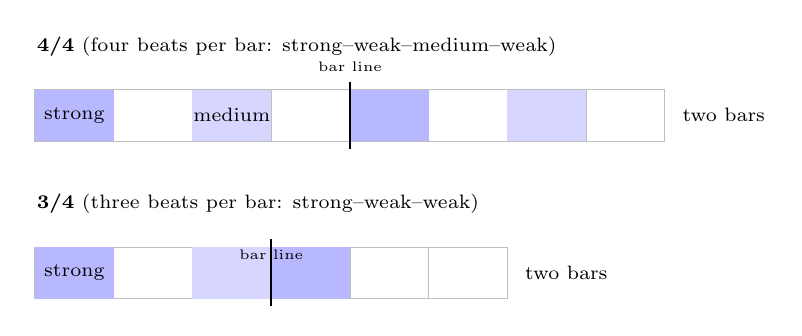
\begin{tikzpicture}[x=1cm,y=1cm,font=\scriptsize]
  \node[anchor=west] at (-0.1,3.2) {\textbf{4/4} (four beats per bar: strong--weak--medium--weak)};
  \foreach \i in {0,...,7} {\draw[black!25] (\i,2) rectangle ++(1,0.65);}
  \fill[blue!28] (0,2) rectangle (1,2.65);
  \fill[blue!16] (2,2) rectangle (3,2.65);
  \fill[blue!28] (4,2) rectangle (5,2.65);
  \fill[blue!16] (6,2) rectangle (7,2.65);
  \node at (0.5,2.33) {strong};
  \node at (2.5,2.33) {medium};
  \draw[thick] (4,1.9) -- (4,2.75) node[above] {\tiny bar line};
  \node[anchor=west] at (8.1,2.33) {two bars};

  \node[anchor=west] at (-0.1,1.2) {\textbf{3/4} (three beats per bar: strong--weak--weak)};
  \foreach \i in {0,...,5} {\draw[black!25] (\i,0) rectangle ++(1,0.65);}
  \fill[blue!28] (0,0) rectangle (1,0.65);
  \fill[blue!16] (2,0) rectangle (3,0.65);
  \fill[blue!28] (3,0) rectangle (4,0.65);
  \node at (0.5,0.33) {strong};
  \draw[thick] (3,-0.1) -- (3,0.75) node[below] {\tiny bar line};
  \node[anchor=west] at (6.1,0.33) {two bars};
\end{tikzpicture}

\small Figure 2-1. Beat groups in 4/4 and 3/4. Shading marks strong/weak positions only; it does not mean you must play at those volumes.
\end{center}

\subsection{Time signature: beats per bar and the beat unit}

A time signature looks like a fraction, but it is not arithmetic:

\begin{itemize}
  \item \textbf{Numerator}: number of beats per bar.
  \item \textbf{Denominator}: which note value counts as one beat: 4 = quarter note, 8 = eighth note, 2 = half note.
\end{itemize}

4/4 means four beats per bar with the quarter note as the beat; 3/4 means three; 2/4 means two. 6/8 is a compound meter: six eighth notes per bar, grouped 3+3, with accents on the first and fourth eighth notes. It feels like ``two beats, each with three subdivisions.''

\begin{center}
\small
\begin{tabular}{llll}
\toprule
Meter & Beats per bar & Beat unit & Typical accents \\
\midrule
4/4 & 4 & quarter note & 1 strong, 3 medium, 2/4 weak \\
3/4 & 3 & quarter note & 1 strong, 2/3 weak (waltz feel) \\
2/4 & 2 & quarter note & 1 strong, 2 weak (march feel) \\
6/8 & 6 eighth notes & eighth note & 1 strong, 4 medium, grouped 3+3 \\
\bottomrule
\end{tabular}

Table 2-1. Four beginner meters. The ``beats'' of 6/8 are often counted as two groups of three in listening.
\end{center}

4/4 and 2/2 (cut time) are relatives, but 2/2 has two beats per bar with the half note as the beat; it feels faster and broader. Do not notate one as the other.

\subsection{Note values: from whole note to sixteenth}

Note values halve step by step from the whole note:

\begin{center}
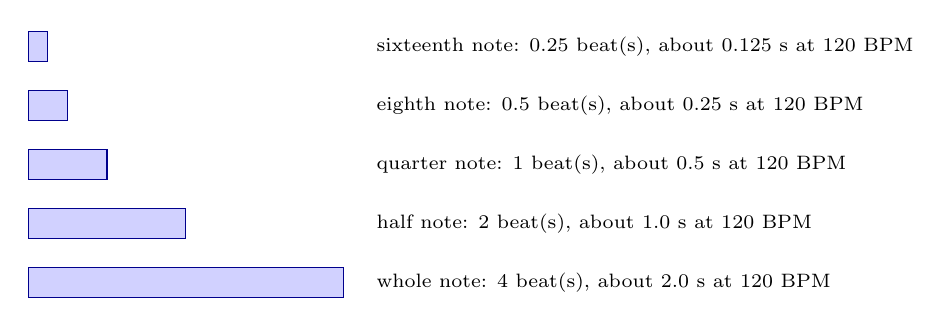
\begin{tikzpicture}[x=1cm,y=1cm,font=\scriptsize]
  \foreach \y/\name/\beats/\sec/\w in {0/whole note/4/2.0/4, 1/half note/2/1.0/2, 2/quarter note/1/0.5/1, 3/eighth note/0.5/0.25/0.5, 4/sixteenth note/0.25/0.125/0.25} {
    \draw[fill=blue!18,draw=blue!55!black] (0,\y*0.75) rectangle ++(\w,0.38);
    \node[anchor=west] at (4.3,\y*0.75+0.19) {\name: \beats\ beat(s), about \sec\ s at 120 BPM};
  }
\end{tikzpicture}

\small Figure 2-2. Relative values of whole, half, quarter, eighth, and sixteenth notes at 120 BPM with the quarter note as one beat.
\end{center}

A dot adds half of the original value: a dotted quarter is 1.5 beats, a dotted half is 3 beats. A tie joins adjacent notes of the same pitch into one longer sound without retriggering; a slur connects different pitches to mark a phrase rather than to add durations. They look similar but do different jobs.

A triplet divides the space of two beats into three equal parts, each 2/3 of a beat; it is a 3-against-2 rhythm, not a change of meter. Beginners should master half, quarter, eighth, and dotted values first; triplets return in Chapter 7.

\subsection{Rests, weak positions, and pickups}

A rest is ``time with no sound,'' not ``no music.'' Whole, half, quarter, and eighth rests last as long as their note counterparts; they still count toward the bar's total duration. Do not drop them because they are silent.

A weak position is a spot inside a beat that does not receive the main accent. An anacrusis (pickup) is a phrase that starts on a weak position and leaves the first bar incomplete. A pickup is not an error: it lets the phrase ``take a step before landing,'' and pop choruses often use one.

Judge strong and weak positions by subdivision, not only by beat number: in 4/4 the first beat is strong, but the second eighth of that beat is weak. Syncopation moves accents onto exactly these weak positions.

\subsection{Syncopation and backbeat}

Syncopation puts the accent on a weak beat or weak position, so the listener feels ``the pulse is there, but the accent is not on the downbeat.'' Two common forms:

\begin{itemize}
  \item \textbf{Backbeat}: in 4/4, accent beats 2 and 4 while 1 and 3 stay lighter; pop drums often put the snare there.
  \item \textbf{Weak-position syncopation}: start on the second half of a beat, or let a note cross the next downbeat, creating a pushed or laid-back feel.
\end{itemize}

\begin{center}
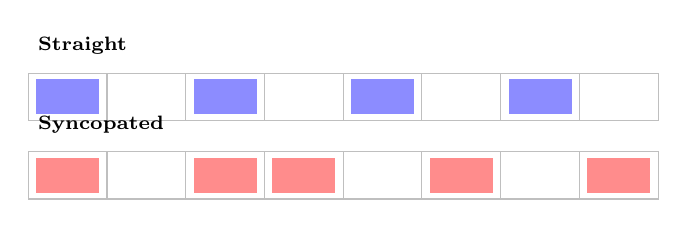
\begin{tikzpicture}[x=1cm,y=1cm,font=\scriptsize]
  \foreach \i in {0,...,7} {\draw[black!25] (\i,1) rectangle ++(1,0.6);}
  \foreach \i in {0,2,4,6} {\fill[blue!45] (\i+0.1,1.08) rectangle ++(0.8,0.44);}
  \node[anchor=west] at (0,1.95) {\textbf{Straight}};

  \foreach \i in {0,...,7} {\draw[black!25] (\i,0) rectangle ++(1,0.6);}
  \foreach \i in {0,2,3,5,7} {\fill[red!45] (\i+0.1,0.08) rectangle ++(0.8,0.44);}
  \node[anchor=west] at (0,0.95) {\textbf{Syncopated}};
\end{tikzpicture}

\small Figure 2-3. Straight and syncopated versions of one 4/4 bar. Top: accents on eighth positions 1, 3, 5, 7; bottom: accents move to weak positions 3, 6, 8. Cells are eighth notes; blocks mark onsets, not equal durations.
\end{center}

Syncopation is not ``playing wrong.'' The test is whether the underlying pulse remains countable after removing the accents. If listeners feel ``the beat is there, the accent moved,'' it is syncopation; if they cannot count at all, the rhythm is simply unaligned.

\subsection{Tempo, groove, and style}

The same notes at different speeds create a different groove. 4/4 at 120 BPM feels steady, 140 BPM feels urgent, 70 BPM feels heavy. Swing performance makes eighth notes long--short rather than equal; straight performance keeps them even. Swing is a performance/arrangement treatment, not a meter change: the score still notates eighth notes, and the treatment lives in performance or processing.

Do not change tempo, meter, and syncopation at the same time. Change one variable at a time: count straight eighths first, add backbeat second, and only then try weak-position syncopation, so your ear can tell where each change comes from.

\subsection{How to do it in Yeban}

\begin{enumerate}
  \item When creating a project, set tempo (BPM), time signature, and sample rate in the startup page's details. The time-signature numerator steps from 1 to 32; the denominator offers 1/2/4/8/16/32. After the project exists, the ruler draws bars and beat lines from that meter.
  \item The transport shows a BPM field; changing it updates both playback speed and bar width. Start between 90 and 120 BPM, where you can count clearly.
  \item The menu has a ``metronome'' toggle. Turn it on and count with the click: four per bar in 4/4, three in 3/4, two groups of three in 6/8. First follow by ear without looking at the screen.
  \item In the arrangement area, read the ruler: vertical lines are bar lines and numbers are bar numbers; zoom in to see beat lines and subdivisions. Before writing a clip, confirm which bar it starts and ends in.
  \item In the piano roll, use the draw tool (number key \texttt{2}); the grid snaps to the current quantization, so fast writing does not drift. To fix hand-played timing, use ``Edit $\rightarrow$ Quantize Notes (1/16).''
  \item Press \texttt{Space} and count with the transport. If accents keep landing on offbeats, first check whether the notes sit in the second half of each beat; do not blame monitoring first.
\end{enumerate}

\screenshot{piano-roll-rhythm-grid}{Piano-roll rhythm grid and time signature}{Piano-roll rhythm grid and time signature}

\textbf{Scope note:} this volume treats swing as a groove and writing concept. The swing parameter in Yeban's drum generator belongs to the instruments/arrangement volumes and is not expanded here. Meter, BPM, and grid operations remain as described in this chapter.

\subsection{Exercises}

\begin{enumerate}
  \item How long is one 4/4 bar at 120 BPM? At 90 BPM?\\
  \emph{Hint:} one beat is 60/BPM seconds; 4/4 has four beats.\\
  \emph{Answer:} 2 s at 120 BPM; \(4 \times 60/90 \approx 2.67\) s at 90 BPM.
  \item 3/4 and 6/8 both often sound ``in groups of three.'' How do their beat counts differ?\\
  \emph{Answer:} 3/4 has three quarter-note beats per bar; 6/8 has six eighth notes grouped 3+3, with accents on the first and fourth eighths.
  \item How many beats is a dotted quarter? A dotted half?\\
  \emph{Answer:} 1.5 beats; 3 beats.
  \item If you turn a straight 4/4 pattern into a backbeat, which beats carry the accent?\\
  \emph{Answer:} beats 2 and 4 (the second and fourth beats of each bar).
  \item In Yeban, create a 4/4 project at 100 BPM, turn on the metronome, and write two bars of eighth notes with a strong--weak--strong--weak pattern; then add a note on the second half of beat 2 in the second bar and listen for syncopation.\\
  \emph{Hint:} Align to the bar line first and count the eight half-cells of each beat; do not guess positions by dragging.
\end{enumerate}

\subsection{Help topic map}

\begin{center}
\footnotesize
\setlength{\tabcolsep}{3pt}
\begin{longtable}{p{0.33\linewidth}p{0.44\linewidth}p{0.17\linewidth}}
\toprule
Section & In-app help anchor & Note \\
\midrule
\endhead
Pulse, beat, and tempo & \texttt{music-theory-pulse-beat-tempo} & concept / Equation \eqref{eq:beat-duration} \\
Time signature & \texttt{music-theory-time-signature} & Table 2-1 \\
Note values & \texttt{music-theory-note-values} & Figure 2-2 \\
Rests, weak positions, pickups & \texttt{music-theory-rests-weak-beats} & concept \\
Syncopation and backbeat & \texttt{music-theory-syncopation-backbeat} & Figure 2-3 \\
Tempo and groove & \texttt{music-theory-groove-tempo} & concept \\
How to do it in Yeban & \texttt{music-theory-timeline-grid} & procedure \\
Exercises & \texttt{music-theory-ch2-practice} & answers above \\
\bottomrule
\end{longtable}
\end{center}
